\documentclass{article}
\usepackage{graphicx}
\usepackage{amsmath}
\usepackage{amssymb}
\usepackage{booktabs}
\usepackage{tabularx}
\usepackage{enumitem}
\usepackage{hyperref}
\usepackage{float}
\usepackage{comment}
\usepackage{titlesec}
\usepackage{algorithm}
\usepackage{algpseudocode}
\usepackage[dvipsnames]{xcolor}
\usepackage[UTF8, scheme=plain]{ctex}
\usepackage[margin=1in]{geometry}
\everymath{\displaystyle}
\linespread{1.2}
\setlength{\parindent}{0em}
\setlength{\parskip}{5pt}
\author{Xiuyuan Lu}

\newenvironment{remark}{\par\noindent\textcolor{PineGreen}{\textbf{Comment: }}\color{PineGreen}\ignorespaces}{\par}



\titleclass{\subsubsubsection}{straight}[\subsection]
\newcounter{subsubsubsection}[subsubsection]
\renewcommand{\thesubsubsubsection}{\thesubsubsection.\arabic{subsubsubsection}}
\titleformat{\subsubsubsection}{\normalfont\normalsize\bfseries}{\thesubsubsubsection}{1em}{}
\titlespacing*{\subsubsubsection}{0pt}{3.25ex plus 1ex minus .2ex}{1em}
\makeatletter
\setcounter{secnumdepth}{4}
\setcounter{tocdepth}{4}
\makeatletter
\newcommand{\l@subsubsubsection}{\@dottedtocline{4}{7em}{4em}}
\makeatother
\makeatother

\title{Innovative IDOCRIW-DOBI-DPC model with KNN-Density and Adaptive Thresholding: An application to transport safety planning for US States}
\begin{document}
\maketitle

\begin{abstract}

\end{abstract}
\begin{remark}
参考文献什么时候写?引用的格式?暂时先用comment放在文中防止忘记.
\end{remark}

\section{Introduction}
Decision-making is one of the most critical and fundamental functions of management, as the achievement of organizational goals heavily depends on its effectiveness. Among various decision-making methodologies, Multiple Criteria Decision Making (MCDM) serves as a comprehensive framework for addressing real-world challenges, particularly due to its ability to deliver stable, reliable, and efficient results, which are qualities essential for effective decision-making. This is especially crucial in fields such as road safety, where robust and well-justified decisions are imperative. However, selecting the most suitable MCDM method from existing models has been a persistent challenge for decision-makers, primarily due to the inherent input sensitivity and uncertainty of these models. Consequently, there is a pressing need to develop advanced MCDM frameworks that minimize such limitations, ensuring high robustness and reliability in decision making.

In doing so, prior researches have laid a solid foundation for MCDM applications in road safety. However, research gaps still remain. First, there remains a lack of universal evaluation frameworks for diverse decision making contexts. Second, most studies focused on single countries or small regions, and the complexities of cross-national diversity in factors such as regulations, infrastructure, and cultural preferences are yet to be accounted for. Third, few studies integrate weighting, aggregation, and clustering into a unified pipeline, though processes like grouping, deconstruction, and decomposition are equally essential. Finally, traditional methods like DPC suffer from manual center selection and noise sensitivity, facing uncertainty in small-to-medium datasets. Addressing these gaps is pivotal for advancing both the theoretical rigor and practical applicability of MCDM frameworks in road safety assessment. 

To this end, the current study integrated IDOCRIW (Integrated Determination of Objective CRIteria Weights), DOBI (DOmbi BonferronI), and DPC (Density Peak Clustering), proposing an innovative model of IDOCRIW-DOBI-DPC enhanced with KNN-density and Adaptive Thresholding. Through the development and application of the model, this study contributes to the industrial community in several ways. 
\begin{itemize}
\item First, a set of regional specific Safety Performance Indicators (SPIs) is constructed, which lays the foundation for the comprehensive assessment of road safety in the United States. 
\item Second, the DPC algorithm is enhanced with KNN-density and Adaptive Thresholding, which balances between automation and performance for practical applications. The modification enhances robustness through KNN-based density estimation and better handles noise via adaptive density thresholds. 
\item Additionally, the study provides insights for US states to formulate future road safety strategies and operational measures, ensuring data-driven and context-aware policy making. 
\end{itemize}
The remainder of this paper is organized as follows: Section 2 review the institutional capacity in road safety management, and the MCDM procedure. Section 3 presents the set of SPIs, as well as data in this study. Section 4 describes the innovative model of IDOCRIW-DOBI-DPC enhanced with KNN-Density and Adaptive Thresholding, while results and robustness analysis are included in Section 5. The practical guidance and implications of this study is discussed in Section 6. Finally, Section 7 summarizes the key findings and research contributions, critically examines the study's limitations, and proposes potential directions for future investigation.

\section{Literature Review}

\subsection{US states institutional compacity in transport safety management}
\begin{remark}
\textit{The Vision Zero Handbook}
https://doi.org/10.1007/978-3-030-76505-7\_19
\end{remark}
Over the past few decades, various organizaitons have been consistently collecting and analyzing road safty data, offering practical guidance to states and cities for specific improvements. \\
On a macro level, \dots \\
On a meso-level, \dots \\
At the micro level, \dots \\
\begin{remark}
Literature Review 的工作量似乎较大\dots 故暂缓.
\end{remark}

\subsection{MCDM procedure}

\subsubsection{Uncertainty of MCDM process}

\subsubsection{DPC applications and limitations}


\subsection{Research gaps}
\begin{remark}
是否和Introduction有重复? 可否删去? \\
或者将MCDM相关的Research gaps放在这一部分?
\end{remark}


\section{Data}
\subsection{Index construction}

\begin{remark}
这个案例中的SPI是怎么定的?
\end{remark}
\begin{figure}[H]
\centering
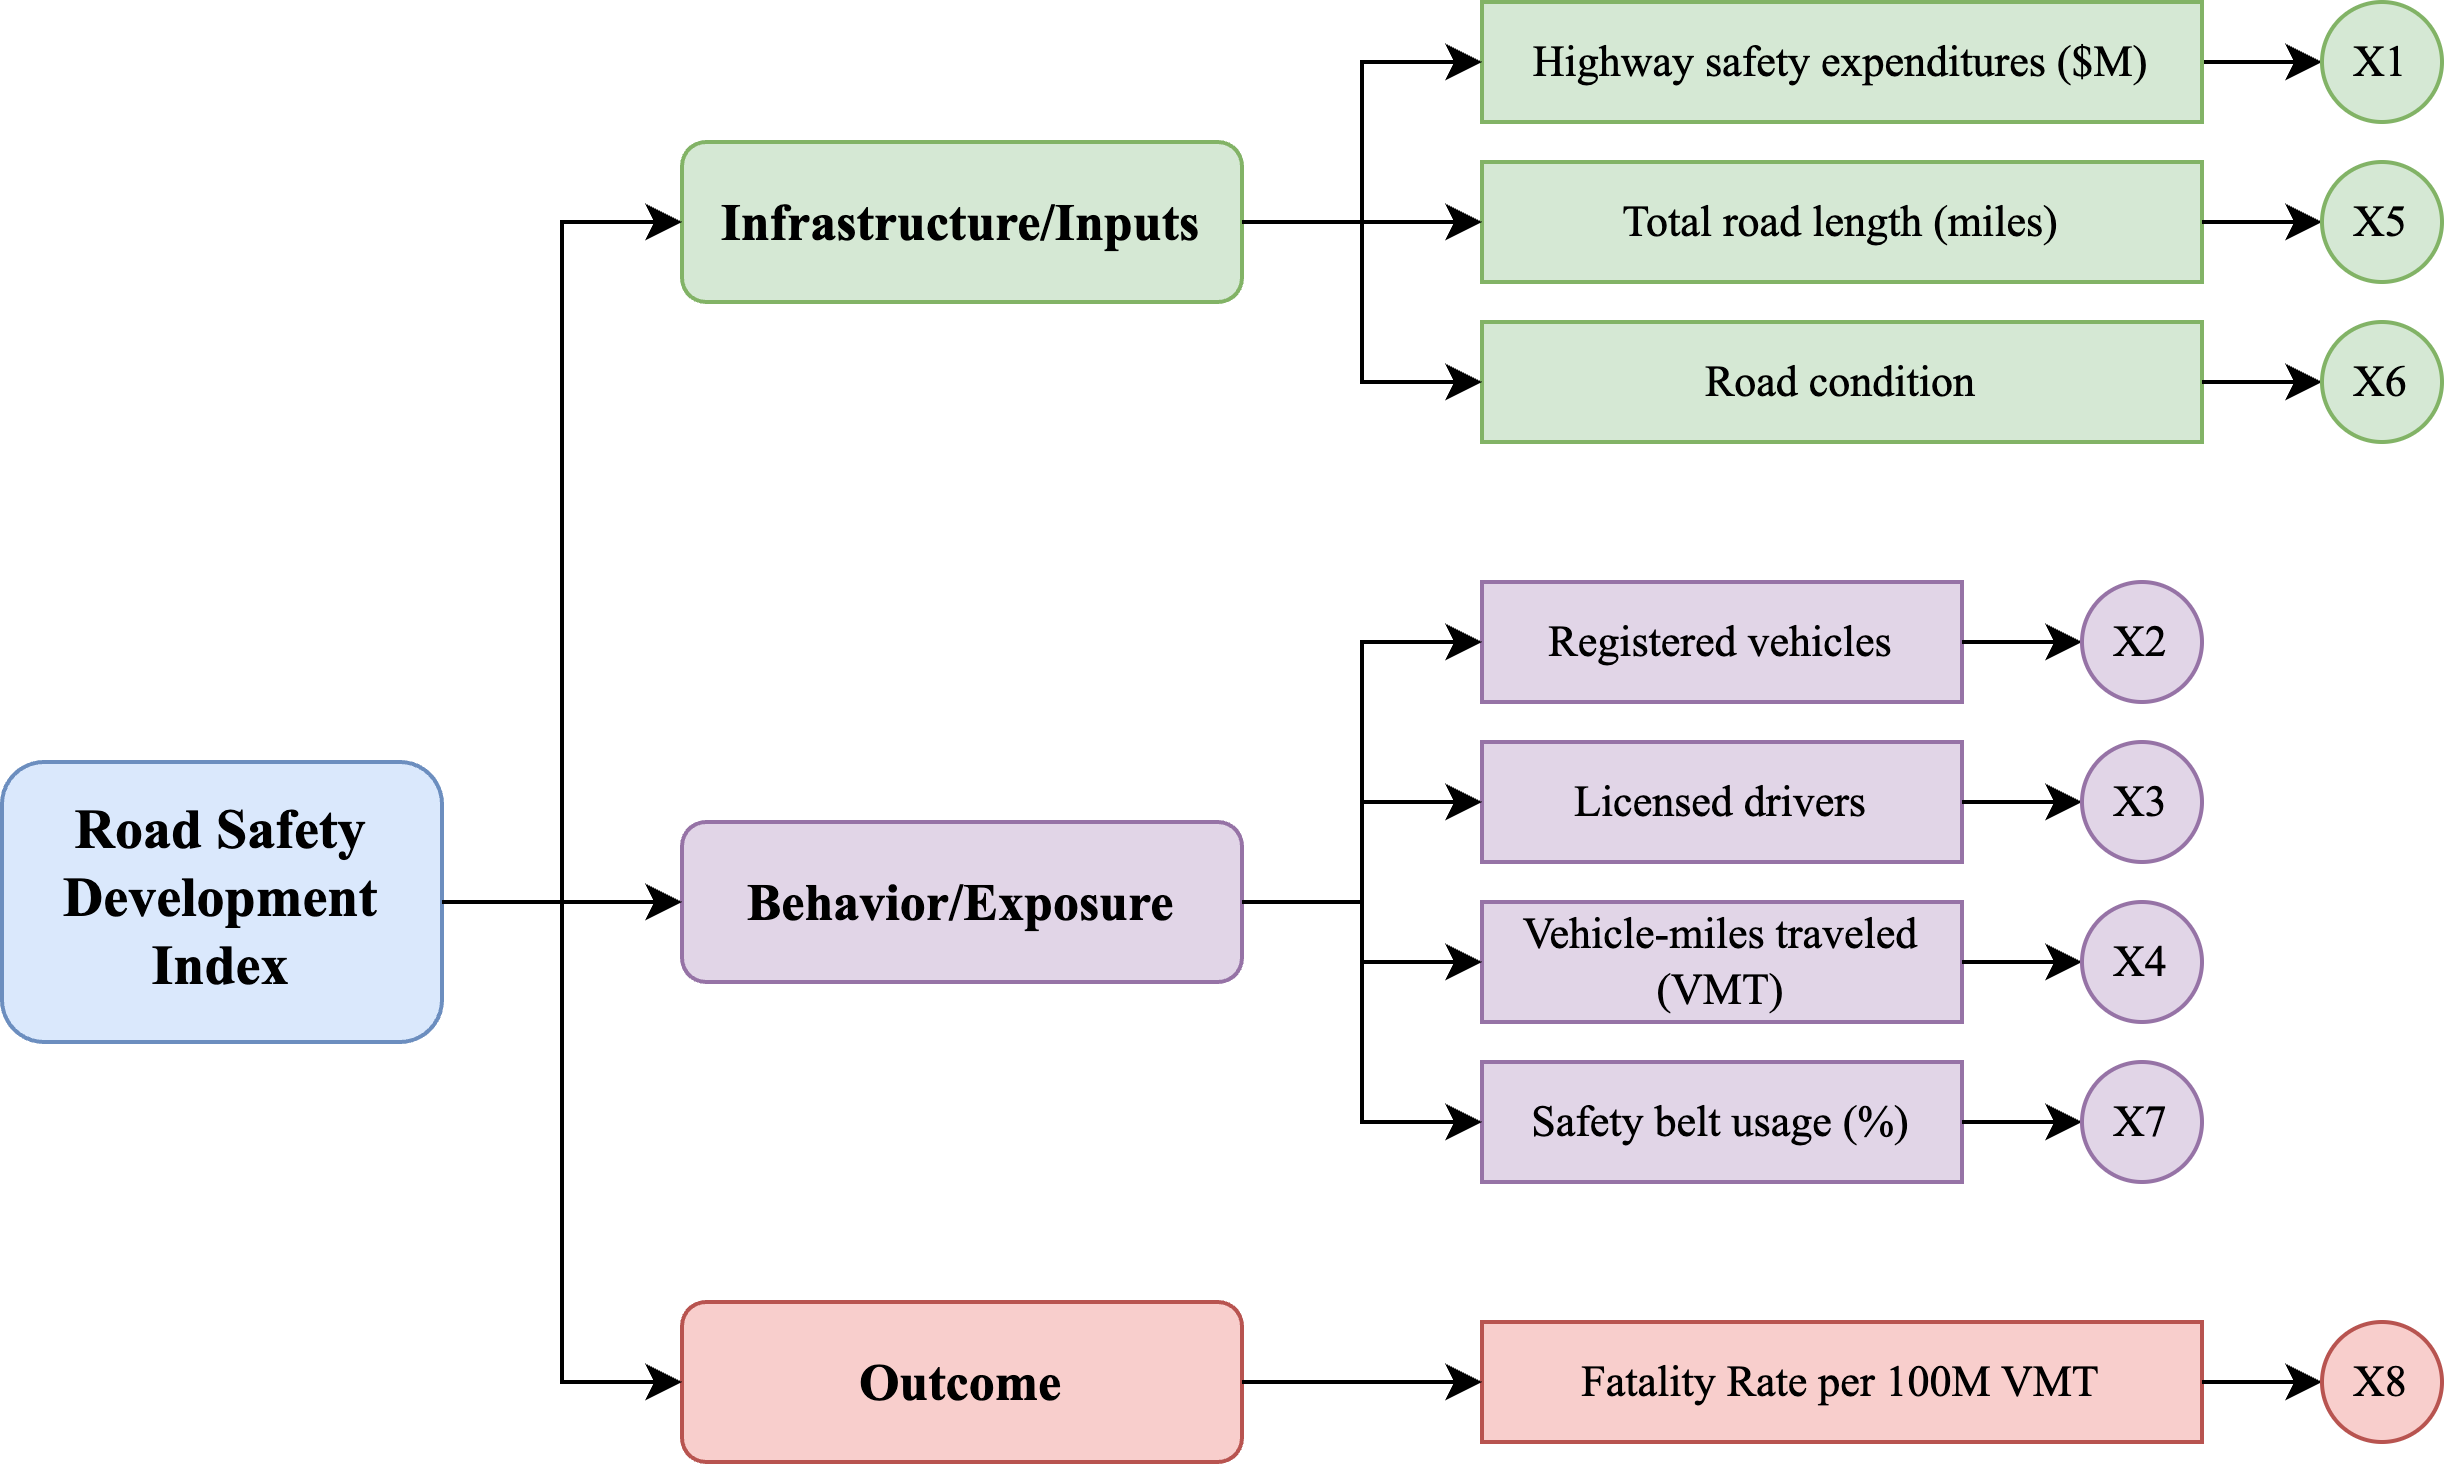
\includegraphics[width=6in]{index.png}
\end{figure}
\begin{remark}
通过draw.io绘制.
\end{remark}
\subsection{Data sources}

交代数据来源
\begin{remark}
    Suggested APA Format Citation:

    National Center for Statistics and Analysis. (2024, December). Traffic safety facts 2022: A compilation of motor vehicle traffic crash data (Report No. DOT HS 813 656). National Highway Traffic Safety Administration.

但是还有一部分数据不是我收集的,需要重新交代数据来源吗?

在另一篇\textit{Measurement of road safety situation by CRITIC-TODIM-NMF: A lesson system of legislation and regulation for the United States}发现其余的数据来自: \\
U.S. Bureau of Transportation Statistics, State Transportation Statistics. 2021, U.S. Bureau of Transportation Statistics (BTS). \\
https://crashstats.nhtsa.dot.gov/Api/Public/ViewPublication/812947 \\
https://crashstats.nhtsa.dot.gov/Api/Public/ViewPublication/811651 \\
National Highway Traffic Safety Administration, Research Testing Databases. 2021, National Highway Traffic Safety Administration (NHTSA).
\end{remark}
\subsection{Data cleaning}

交代数据的预处理（奇异值剔除、缺失值替换）
\begin{remark}
没有遇到缺失值是不是这一部分就不用写了?
\end{remark}
\section{Methodology}
\subsection{IDOCRIW}
\begin{remark}
Original: \textit{The Recalculation of the Weights of Criteria in MCDM Methods Using the Bayes Approach}\\
https://doi.org/10.3390/sym10060205

Where I got the summarized version of the IDOCRIW workflow: \textit{MADM} \\
https://doi.org/10.1007/978-3-030-15009-9
\end{remark}
The IDOCRIW method, developed by Zavadskas and Podvezko in 2016, was formulated as an advanced hybrid weighting technique for solving MCDM challenges. This approach seeks to overcome the shortcomings of conventional weighting methods by integrating two complementary objective techniques—Entropy and CILOS—to deliver more comprehensive and reliable criterion weights. It specifically addresses the limitations of single-method approaches by simultaneously considering data dispersion and criterion interdependencies, while also handling both positive and negative attribute values through systematic normalization.

The IDOCRIW method demonstrates distinct advantages compared to standalone weighting techniques like Entropy or CILOS. First, it mitigates subjective bias through its dual-objective foundation, whereas traditional Entropy weights may overlook criterion interactions. Second, its compensatory nature allows for balanced trade-offs between attributes—a feature absent in non-compensatory methods. Unlike basic normalization techniques, IDOCRIW's square matrix transformation and impact loss calculation provide robust handling of extreme values while preserving subtle data variations. Under identical conditions, this hybrid approach yields more nuanced weight distributions than either Entropy or CILOS applied independently, particularly in datasets with conflicting criterion priorities.

The steps in the IDOCRIW method are as follows:
\begin{enumerate}[label=~\alph*)]
\item An initial decision matrix is constructed, where each row represents an alternative and each column represents a criterion. 
\item The initial decision matrix is normalized through the vector normalization technique. 
\item Compute the degree of entropy and derive entropy weights. 
\item Construct a square matrix using the best-performing alternative for each criterion to establish benchmark values.
\item Compute the performance degradation of non-optimal alternatives relative to the benchmark for each criterion, then organize impact losses into a matrix to model trade-offs between criteria when prioritizing one over others.
\item Solve the weight system matrix to derive secondary weights that account for criterion interdependencies.
\item Combine entropy and CILOS weights into final weights, balancing data dispersion and criterion interactions.
\end{enumerate}


\subsection{DOBI}
\begin{remark}
https://doi.org/10.1016/j.omega.2022.102690
\end{remark}
The DOmbi Bonferroni (DOBI) method is a novel multi-criteria decision-making (MCDM) technique that integrates Dombi norms and Bonferroni mean operators to address uncertainty, model interdependencies between criteria, and adapt to decision-makers' risk preferences. Unlike traditional linear methods, DOBI employs nonlinear aggregation to better reflect real-world trade-offs while preserving data proportionality during normalization, avoiding distortions common in approaches like TOPSIS or MABAC. Its adjustable parameters allow simulation of risk scenarios, ensuring robust rankings resistant to extreme values. In applications such as sustainability assessment, DOBI balances complex criteria interactions—demonstrated in banking sector evaluations where it identified top performers by dynamically weighting economic, social, and environmental factors. The method's flexibility and stability make it particularly suited for problems requiring nuanced trade-offs and adaptive decision-making frameworks.

\begin{remark}
To be continued. 
\end{remark}

\subsection{DPC Enhanced with KNN-Density and Adaptive Thresholding (KAT-DPC)}
\begin{remark}
\textit{Clustering by fast search and find of density peaks}\\
https://www.science.org/doi/10.1126/science.1242072
\end{remark}
Density Peaks Clustering (DPC), introduced by Rodriguez and Laio in 2014, is a powerful clustering algorithm that identifies cluster centers as points with high local density ($\rho$) and large separation ($\delta$) from other high-density points. Unlike traditional centroid-based or hierarchical methods, DPC excels in detecting arbitrarily shaped clusters and automatically distinguishing noise points without requiring predefined cluster numbers. 

However, the original DPC has limitations, including reliance on manual selection of cluster centers from a decision graph ($\rho$ vs. $\delta$) and sensitivity to the cutoff distance ($d_c$) in density estimation, similar to DBSCAN’s $\varepsilon$ challenge. These factors can introduce instability in clustering results, particularly in noisy or high-dimensional datasets where distance metrics lose meaning. Despite these challenges, DPC remains a powerful tool for unsupervised learning, particularly in applications like bioinformatics, image analysis, and anomaly detection, where cluster shapes and noise resilience are critical. Various studies have proposed improvements to the Density Peaks Clustering (DPC) algorithm to address its limitations, such as parameter sensitivity, scalability, and performance in high-dimensional or complex datasets. 

The k-Nearest Neighbors (KNN) algorithm is a non-parametric classification method rooted in early pattern recognition research. Introduced conceptually by Fix and Hodges (1951) and formalized by Cover and Hart (1967), KNN operates on a simple principle: an unclassified data point is assigned the label most frequent among its $k$ closest neighbors in a labeled training set. The algorithm requires no assumptions about underlying data distributions, making it versatile but reliant on a meaningful distance metric. KNN's effectiveness hinges on local data density and the choice of $k$, balancing bias-variance trade-offs. Despite its simplicity, KNN remains widely used for its interpretability and adaptability to complex decision boundaries.

\subsection{Innovative IDOCRIW-DOBI-DPC with KNN-Density and Adaptive Thresholding}
\begin{enumerate}[label=\textbf{Step}~\arabic*]
\item Construct the decision matrix.\\
\[A=
\begin{bmatrix}
a_{11} & a_{12} & \cdots & a_{1n} \\
a_{21} & a_{22} & \cdots & a_{2n} \\
\vdots & \vdots & \ddots & \vdots \\
a_{m1} & a_{m2} & \cdots & a_{mn} \\
\end{bmatrix}_{m \times n}.\]
where $a_{ij}$ represents the $j$th criterion value of the $i$th alternative.
\item Normalize the decision matrix by means of vector normalization.
\begin{enumerate}
\item For cost criteria ($X8$ in this case study):
\[b_{ij} = \frac{\frac{1}{a_{ij}}}{\sqrt{\sum_{i=1}^{m} (\frac{1}{a_{ij}})^{2}}}.\]
\item For benefit criteria ($X1-X7$):
\[b_{ij} = \frac{a_{ij}}{\sqrt{\sum_{i=1}^{m} a_{ij}^{2}}}.\]
\end{enumerate}
Where $b_{ij}$ is the normalized performance value of the $j$th criterion value of the $i$th alternative. Therefore, we arrive at the normalized decision matrix:
\[B = 
\begin{bmatrix}
    b_{11} & b_{12} & \cdots & b_{1n} \\
    b_{21} & b_{22} & \cdots & b_{2n} \\
    \vdots & \vdots & \ddots & \vdots \\
    b_{m1} & b_{m2} & \cdots & b_{mn} \\
    \end{bmatrix}_{m \times n}.\]
\item Assign the weights to the criterion with IDOCRIW.\\
The weights are calculated using the following equation:
\[\omega _{j} = \frac{q_{j} \cdot w_{j}}{\sum_{j=1}^{n} q_{j} \cdot w_{j}}\]
where $q$ represents the CILOS weights and $w$ represents the entropy weights. 
\begin{remark}
需要完整写出计算用到的所有公式吗?? 即,计算公式出现在这一部分,步骤描述出现在4.1, 但IDOCRIW的计算公式较多,如果在这里罗列是否过于冗长? 可否通过引用entropy和CILOS的文献省略公式?
\end{remark}
The CILOS weight $q$ is determined through the solution of the following equation:
\[
\begin{bmatrix}{}
-\sum_{i=1}^{n} p_{i1} & p_{12} & \dots & p_{1n} \\
p_{21}  & -\sum_{i=1}^{n} p_{i2} & \dots & p_{2n} \\
\vdots  & \vdots & \ddots & \vdots \\
p_{n1}  & p_{n2} & \dots & -\sum_{i=1}^{n} p_{in}
\end{bmatrix}
q^{T} = 0,\]
where $p_{ij}$ represents the impact loss of the $j$th attribute, if selected as the best value. 
The entropy weight $w$ is computed through the following equation:
\[w_{j} = \frac{1-E_{j}}{\sum_{j=1}^{n} (1-E_{j})},\]
where $E_{j} = -\frac{1}{\ln n} \sum_{i=1}^{n} b_{ij} \cdot \ln b_{ij}$
\item Aggregate the performance with DOBI method.
\begin{enumerate}[label=(\arabic*)]
    \item Dombi-Bonferroni functions:\\
    Weighted Averaging Function (Z1)
    \[Z1_i = \frac{\sum_{j=1}^n b_{ij}}{1 + \left[\frac{\sum_{j=1}^n \sum_{\substack{k=1 \\ k \neq j}}^n \frac{\omega_j \omega_k}{1-w_j} \left(\psi_1 \left(\frac{1-f_{ij}}{f_{ij}}\right)^\zeta + \psi_2 \left(\frac{1-f_{ik}}{f_{ik}}\right)^\zeta\right)}{\psi_1 + \psi_2}\right]^{1/\zeta}}\]
    Weighted Geometric Function (Z2)
    \[Z2_i = \frac{\sum_{j=1}^n b_{ij}}{1 + \left[\frac{\sum_{j=1}^n \sum_{\substack{k=1 \\ k \neq j}}^n \frac{\omega_j \omega_k}{1-w_j} \left(\psi_1 \left(\frac{f_{ij}}{1-f_{ij}}\right)^\zeta + \psi_2 \left(\frac{f_{ik}}{1-f_{ik}}\right)^\zeta\right)}{\psi_1 + \psi_2}\right]^{1/\zeta}}\]
    where $f_{ij} = \frac{b_{ij}}{\sum_{j=1}^n b_{ij}}$.
    
    \item Integrated DOBI value:
    \[\Re_i = \frac{Z1_i + Z2_i}{1 + \frac{1}{2}\left[\left(\frac{1-Z1_i}{Z1_i}\right)^\delta + \left(\frac{1-Z2_i}{Z2_i}\right)^\delta\right]}\]
    
\end{enumerate}
The integrated DOBI values ($\Re_{i}$) are ranked in descending order to obtain the final ranking. 
\item KNN-based density estimation.
\[\rho_i = \frac{1}{\text{mean}(d_{i,\text{KNN}})}\]

\item Delta calculation. 
\[\delta_i = 
\begin{cases} 
    \min_{j:\rho_j > \rho_i}(d_{ij}) & \text{if } \exists j \text{ s.t. } \rho_j > \rho_i \\
    \max_j(d_{ij}) & \text{otherwise}
\end{cases}\]

\item Automated center selection. 
\[\gamma_i = \rho_i \times \delta_i\]
Then sort $\gamma_{i}$ in descending order and use KneeLocator to find the elbow point. The points before the elbow point are selected as cluster centers.

\item Assign clusters using K-means initialization. In case some points are not assigned to any cluster, we reassign them to the nearest cluster center.



\end{enumerate}

\section{Results and Discussion}
\subsection{Computational Results}
\subsubsection{Ranking}
Based on the proposed model, the transport safety scores and corresponding rankings of U.S. states are analyzed across multiple years (2016, 2019, 2022). The results reveal distinct patterns in performance and stability. California (CA), Texas (TX), and Florida (FL) consistently rank among the top states, demonstrating robust transport safety performance. California maintains its leading position across all years, while Texas and Florida show minor fluctuations but remain in the top tier. The District of Columbia (DC), Alaska (AK), and Vermont (VT) persistently rank at the bottom, indicating significant challenges in transport safety. Their scores show minimal improvement over time, suggesting systemic issues that require targeted interventions. 

\subsubsection{Grouping}
To facilitate a meaningful comparative analysis and identify trends in state-level performance, the U.S. states were categorized into distinct groups based on their transport safety scores. The results reveal a clear stratification, with certain states consistently maintaining the highest rankings (e.g., CA, FL, TX, IL, PA) and others persistently occupying the lowest tiers (e.g., AK, DE, DC, HI, VT). Notably, a subset of states, such as UT, VA, and WV, exhibited significant variability in their group assignments over time, suggesting dynamic or unstable performance. These findings enable targeted benchmarking, allowing policymakers to derive insights from top-performing states while investigating the factors contributing to volatility in others.


\subsection{Robustness Test}
\subsubsection{Comparison of Ranking}
\subsubsubsection{Initial Sensitivity}
\subsubsubsection{Intermediate Uncertainty}
\subsubsubsection{Transverse Stability}
\subsubsection{Comparison of Grouping}
\subsubsubsection{Initial Sensitivity}
\subsubsubsection{Intermediate Uncertainty}
\subsubsubsection{Transverse Stability}
\section{Practical Guidance}
\subsection{Dynamic changes of indicators}
\subsection{De-construction of composite index}
\subsection{De-composition of score changes}
\subsection{Benchmarking}
\section{Conclusions and Further Studies}
\section*{References}


\maketitle
\end{document}

